%-- coding:UTF-8 --
\documentclass{article}

\usepackage[english]{babel}
\usepackage[UTF8]{ctex}

\usepackage[letterpaper,top=2cm,bottom=2cm,left=3cm,right=3cm,marginparwidth=1.75cm]{geometry}

\usepackage{amsmath}
\usepackage{graphicx}
\usepackage[colorlinks=true, allcolors=blue]{hyperref}
\usepackage{booktabs}
\usepackage{tabularx}
\usepackage{multirow}
\usepackage{listings}
\usepackage{minted}
\usepackage{xcolor}

\lstdefinestyle{myStyle}{
    backgroundcolor=\color{gray!10}, % 设定背景颜色
    basicstyle=\ttfamily, % 设置基本字体
%    frame=single, % 添加框架
%    rulecolor=\color{black}, % 框架颜色
    keywordstyle=\color{blue}, % 关键字颜色
    commentstyle=\color{green}, % 注释颜色
    stringstyle=\color{red} % 字符串颜色
}


\title{实验3:命令行环境/Python入门基础/Python视觉应用}
\author{方欣 23020007021}
\date{}

\begin{document}
\maketitle

\url{https://github.com/nixgnaf/SDT_report.github.io}

\section{命令行环境}

\subsection{任务控制}
\subsubsection{(1)在终端中执行 sleep 10000 这个任务。然后用 Ctrl-Z 将其切换到后台并使用 bg来继续允许它。现在,使用 pgrep 来查找 pid 并使用 pkill 结束进程而不需要手动输入pid。}

\noindent sleep 10000: 将使终端挂起 10000 秒。\\
Ctrl-Z: 发送 SIGTSTP 信号到当前前台进程,暂停它的执行,并将其放置在后台。\\
bg:将一个或多个暂停的进程恢复到后台继续运行。\\
pgrep:查找匹配特定模式的进程 ID。-f:匹配整个命令行(而不仅仅是进程名称)。\\
pkill:向所有命令行中包含 sleep 的进程发送信号SIGTERM,请求终止进程。
\begin{figure}[h]
    \centering
    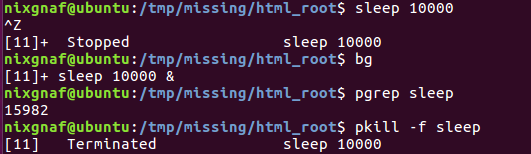
\includegraphics[width=0.5\linewidth]{image1.png}
\end{figure}

\subsubsection{(2)请编写一个 bash 函数 pidwait ,它接受一个 pid 作为输入参数,然后一直等待直到该进程结束。您需要使用 sleep 来避免浪费 CPU 性能。}
\begin{lstlisting}[style=myStyle]
pidwait()
{
   while kill -0 $1 
   do
   sleep 1 
   done
   ls
}
\end{lstlisting}
kill -0 \$1 是一个用于检测进程是否存在的命令。kill -0 不会实际发送信号,但会返回进程是否存在的状态。如果进程存在,它返回 true,否则返回 false。
\$1 是传递给函数的第一个参数,表示待检测的进程 ID (PID)。
\begin{figure}[h]
    \centering
    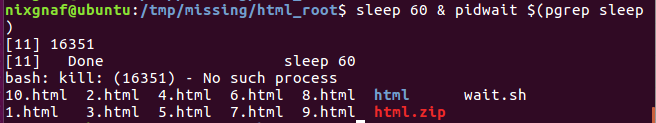
\includegraphics[width=0.75\linewidth]{image2.png}
\end{figure}

\subsection{终端多路复用}

\subsubsection{(3)请完成tmux教程,参考这些步骤来学习如何自定义tmux。}
\noindent tmux new -s session\_name:创建一个带有指定名称的新会话\\
tmux ls:列出所有会话\\
tmux attach -t session\_name:附加到现有会话\\
分离会话:Ctrl-b d\\
关闭会话:exit\\
创建新窗口:Ctrl-b c\\
切换窗口:Ctrl-b n(窗口编号)\\
水平分割面板:Ctrl-b "\\
垂直分割面板:Ctrl-b \%\\
切换面板:Ctrl-b <arrow key>\\
调整面板大小:Ctrl-b Ctrl-<arrow key>\\

\begin{figure}[h]
    \centering
    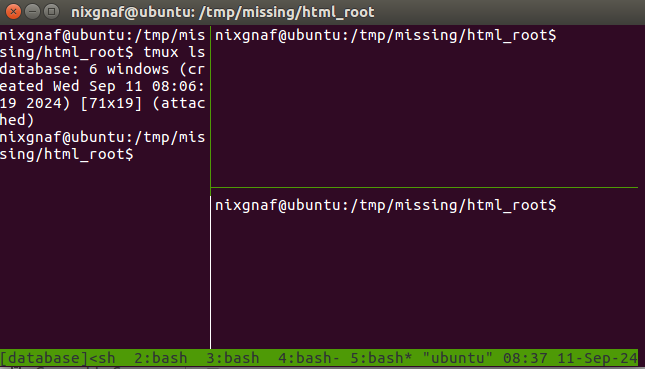
\includegraphics[width=0.75\linewidth]{image3.png}
\end{figure}

\noindent tmux set -g mouse on:开启鼠标控制\\
使用 Alt 键加方向键(箭头)在 tmux 面板之间快速切换的快捷键:
\begin{lstlisting}[style=myStyle]
tmux bind -n M-Left select-pane -L
tmux bind -n M-Right select-pane -R
tmux bind -n M-Up select-pane -U
tmux bind -n M-Down select-pane -D
\end{lstlisting}

\subsection{别名}

\subsubsection{(4)创建一个 dc 别名,它的功能是当我们错误的将 cd 输入为 dc 时也能正确执行。}
\begin{figure}[h]
    \centering
    
\includegraphics[width=0.75\linewidth]{image4.png}
\end{figure}
\begin{figure}[h]
    \centering
    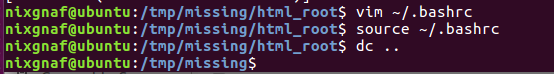
\includegraphics[width=0.75\linewidth]{image5.png}
\end{figure}

\subsubsection{(5)执行 history | awk '{\$1="";print substr(\$0,2)}' | sort | uniq -c | sort -n | tail -n 10 来获取您最常用的十条命令,尝试为它们创建别名。}
\noindent 在 ~/.bashrc文件中使用alias添加对应别名。
\begin{figure}[h]
    \centering
    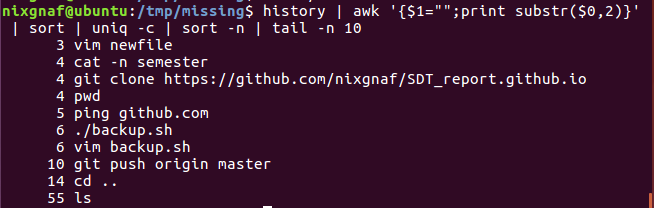
\includegraphics[width=0.75\linewidth]{image6.png}
\end{figure}

\subsection{配置文件}

\subsubsection{(6)为您的配置文件新建一个文件夹,并设置好版本控制,在其中添加至少一个配置文件,比如说您的 shell,在其中包含一些自定义设置(可以从设置 \$PS1 开始)。}
\begin{lstlisting}[style=myStyle]
 mkdir ~/gits/dotfiles
 git init ~/gits/dotfiles
# 将本机的配置文件,如 .vimrc/.bashrc/.tmux.conf 等复制进该目录
ls -a ~/gits/dotfiles
\end{lstlisting}

\begin{figure}[h]
    \centering
    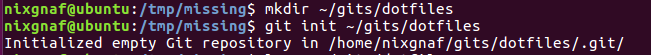
\includegraphics[width=0.75\linewidth]{image7.png}
\end{figure}

\newpage
\subsubsection{(7)建立一种在新设备进行快速安装配置的方法。最简单的方法是写一个shell脚本对每个文件使用 ln -s,也可以使用专用工具在新的虚拟机上测试该安装脚本。}
\lstinputlisting[style=myStyle]{autoconfig.sh}
\noindent 脚本作用:自动创建软链接,使你在新设备上能快速使用相同的配置文件,而无需手动复制或修改。\\
files=\$(ls -a \$1 | grep -E '.[\^.]+' | grep -v .git):列出 \$1 目录中的所有文件(排除 .git 目录和 .、.. 目录)。\$1 是脚本的第一个参数,即配置文件所在的目录。\\
for file in \textbackslash echo \$files`:遍历 \$files` 中的每一个文件。\\
ln -s \$1/\$file ~/\$file:为每个文件创建一个软链接,将其链接到主目录(~)。

\subsubsection{(8)将您现有的所有配置文件移动到项目仓库里。 将项目发布到GitHub。}
\begin{figure}[h]
    \centering
    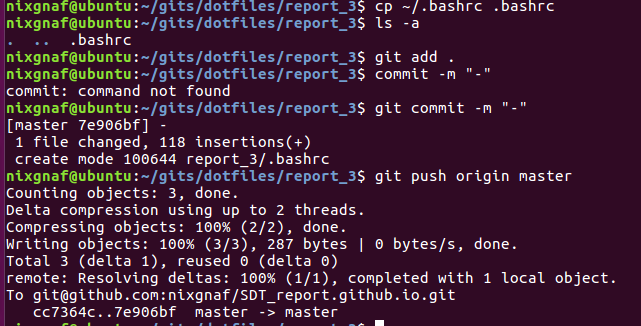
\includegraphics[width=0.7\linewidth]{image8.png}
\end{figure}

\subsection{远端设备}

\noindent 本次实验中在VMware 上从一台虚拟机 SSH 登录到另一台虚拟机。

\subsubsection{(9)前往 ~/.ssh/ 并查看是否已经存在 SSH 密钥对。如果不存在,请使用ssh-keygen -o -a 100 -t ed25519来创建一个。}
\noindent 这里曾经配置过ssh密钥推送到github,直接使用。
\begin{figure}[h]
    \centering
    
\includegraphics[width=0.7\linewidth]{image9.png}
\end{figure}

\subsubsection{(10)在.ssh/config加入下面内容}
\noindent 它将公钥添加到远程主机的\~/.ssh/authorized\_keys 文件中。这允许你通过 SSH 连接到远程主机而无需输入密码。这里将usename和ip改成目标虚拟机的用户名和ip地址。
\begin{lstlisting}[style=myStyle]
Host vm
   User username_goes_here
   HostName ip_goes_here
   IdentityFile ~/.ssh/id_ed25519
   LocalForward 9999 localhost:8888
\end{lstlisting}
\begin{figure}[h]
    \centering
    
\includegraphics[width=0.5\linewidth]{image10.png}
\end{figure}

\subsubsection{(11)使用 ssh-copy-id vm 将您的 ssh 密钥拷贝到服务器。}

\begin{figure}[h]
    \centering
    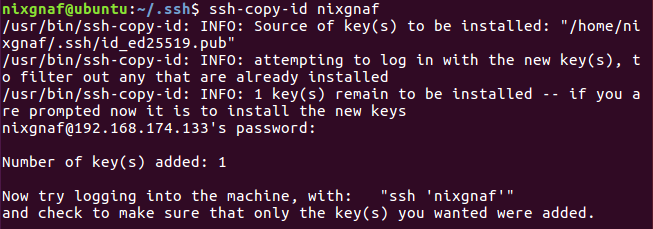
\includegraphics[width=0.75\linewidth]{image11.png}
\end{figure}
\noindent 随后可以直接使用ssh pi进行免密登录
\begin{figure}[h]
    \centering
    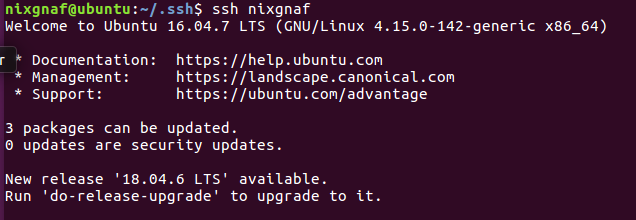
\includegraphics[width=0.75\linewidth]{image12.png}
\end{figure}

\newpage
\subsubsection{(12)使用python -m http.server 8888在您的虚拟机中启动一个 Web 服务器并通过本机的http://localhost:9999 访问虚拟机上的 Web 服务器 }
\begin{figure}[h]
    \centering
    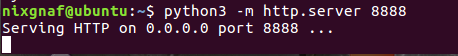
\includegraphics[width=0.75\linewidth]{image13.png}
\end{figure}
\noindent 如图,在源虚拟机上打开浏览器并访问http://localhost:9999显示出目标虚拟机当前工作目录的文件列表。
\begin{figure}[h]
    \centering
    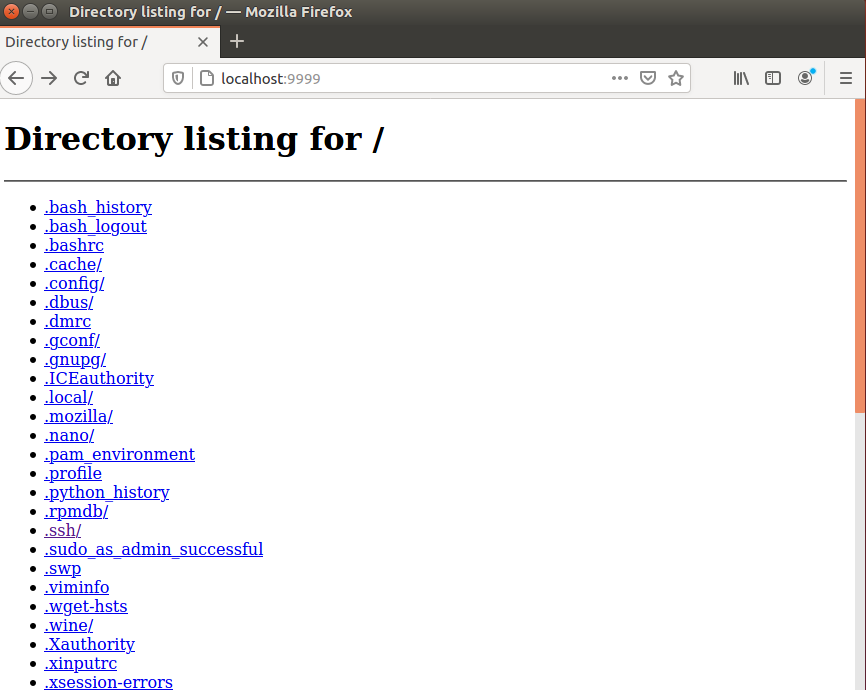
\includegraphics[width=0.75\linewidth]{image14.png}
\end{figure}

\noindent 目标虚拟机上记录了源虚拟机的请求。

\begin{figure}[h]
    \centering
    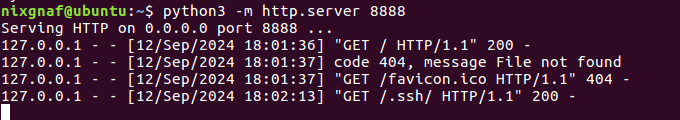
\includegraphics[width=0.75\linewidth]{image15.png}
\end{figure}

\newpage
\section{Python实例}

\subsection{(13)逆序输出数组}
\lstinputlisting[style=myStyle]{reverse.py}
\begin{figure}[h]
    \centering
    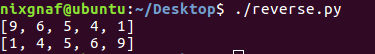
\includegraphics[width=0.5\linewidth]{image17.png}
\end{figure}

\subsection{(14)回文数}
\lstinputlisting[style=myStyle]{palindrome.py}
\begin{figure}[h]
    \centering
    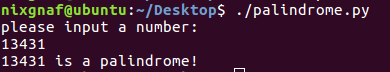
\includegraphics[width=0.5\linewidth]{image18.png}
\end{figure}

\subsection{(15)分解质因数}
\lstinputlisting[style=myStyle]{reduceNum.py}
\begin{figure}[h]
    \centering
    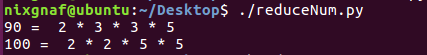
\includegraphics[width=0.5\linewidth]{image16.png}
\end{figure}

\subsection{(16)lambda}
\lstinputlisting[style=myStyle]{lambda.py}
\begin{figure}[h]
    \centering
    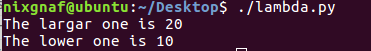
\includegraphics[width=0.5\linewidth]{image19.png}
\end{figure}

\subsection{(17)大写字符串并保存到文件}
\lstinputlisting[style=myStyle]{text.py}
\begin{figure}[h]
    \centering
    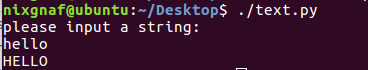
\includegraphics[width=0.5\linewidth]{image21.png}
\end{figure}

\subsection{(18)矩阵相加}
\lstinputlisting[style=myStyle]{matrix.py}
\begin{figure}[h]
    \centering
    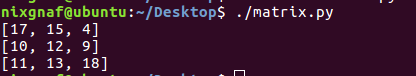
\includegraphics[width=0.5\linewidth]{image22.png}
\end{figure}

\subsection{(19)堆排序}
\lstinputlisting[style=myStyle]{heapSort.py}
\begin{figure}[h]
    \centering
    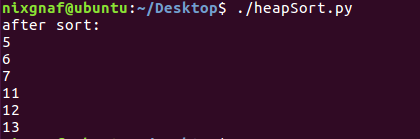
\includegraphics[width=0.5\linewidth]{image23.png}
\end{figure}

\subsection{(20)归并排序}
\lstinputlisting[style=myStyle]{mergeSort.py}
\begin{figure}[h]
    \centering
    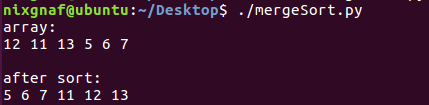
\includegraphics[width=0.5\linewidth]{image24.png}
\end{figure}

\section{Python视觉应用实例}

\subsubsection{(21)PIL:转换灰度图像}
\lstinputlisting[style=myStyle]{1.py}
\begin{figure}[h]
    \centering
    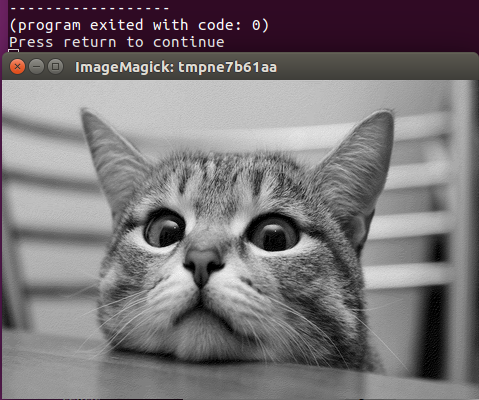
\includegraphics[width=0.5\linewidth]{image25.png}
\end{figure}

\subsubsection{(22)Matplotlib库:图像轮廓和直方图}
\lstinputlisting[style=myStyle]{2.py}
\begin{figure}[h]
    \centering
    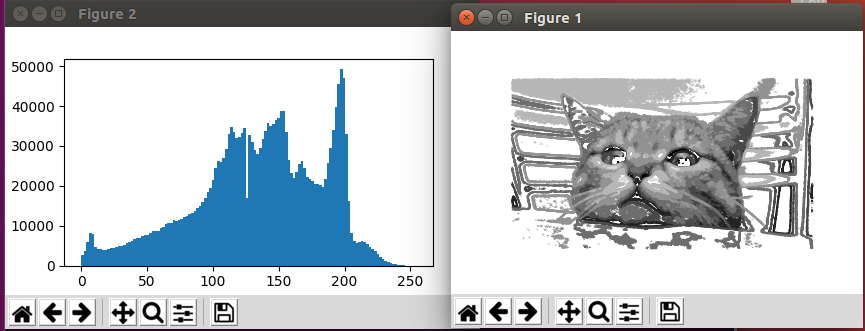
\includegraphics[width=0.75\linewidth]{image26.png}
\end{figure}

\subsection{(23)Numpy:灰度变换}
\lstinputlisting[style=myStyle]{3.py}
\begin{figure}[h]
    \centering
    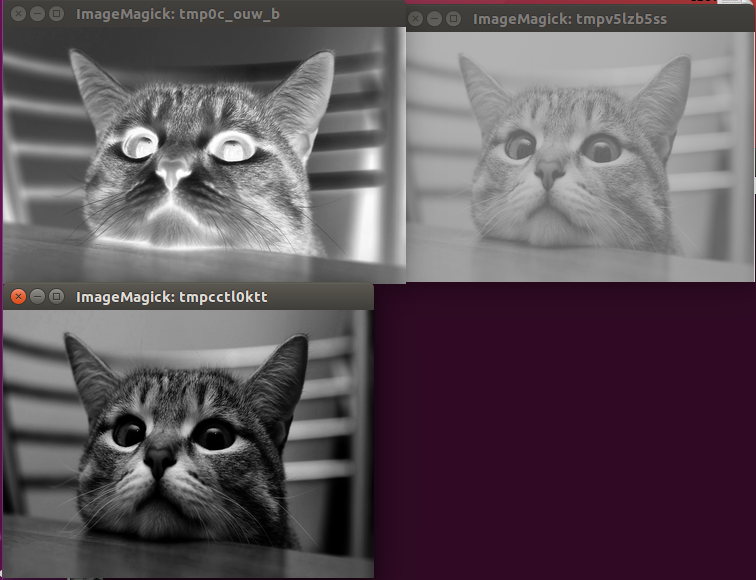
\includegraphics[width=0.75\linewidth]{image27.png}
\end{figure}

\subsection{(24)Scipy:高斯模糊}
\lstinputlisting[style=myStyle]{4.py}
\begin{figure}[h]
    \centering
    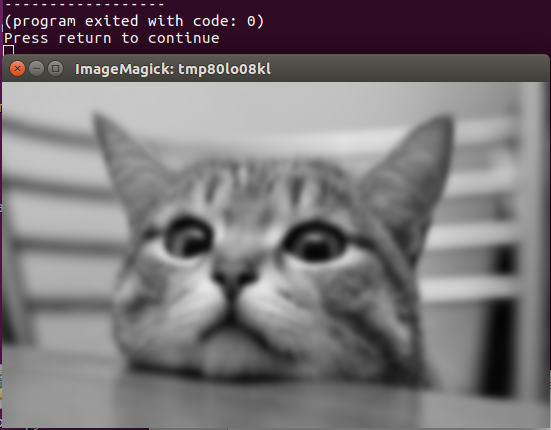
\includegraphics[width=0.5\linewidth]{image28.png}
\end{figure}

\section{结论和心得}
通过本次实验,我学习到了改善shell及其他工具的工作流的方法,以及如何使用SSH操作远端机器。通过Python入门基础,我了解了Python语法知识,并在Python视觉应用中直观感受到图像处理的过程。
\end{document}

